% Kompiuterijos katedros šablonas
% Template of Department of Computer Science II
% Versija 1.0 2015 m. kovas [ March, 2015]

\documentclass[a4paper,12pt,fleqn]{article}
\usepackage[unicode,colorlinks=false]{hyperref}


\usepackage[utf8x]{inputenc}
%

\usepackage[L7x]{fontenc}
\usepackage{times}
\usepackage{ucs}

 %package to switch the language
\usepackage{etoolbox}

  %set up of the page margins
\usepackage[top=2cm, bottom=2cm, left=3cm, right=1.5cm]{geometry}

 %1.1 line spacing
\linespread{1.1}


  %page numbering at the right side
\usepackage{fancyhdr}
\pagestyle{fancyplain}
\fancyhf{}
\renewcommand{\headrulewidth}{0pt} 
\fancyhfoffset[RO]{0cm}

  %to number at the bottom (exchange lines to number at the top)
\rfoot{\thepage}
  %\rhead{\thepage} %

% \usepackage[usenames,dvipsnames]{pstricks}
\urlstyle{same}
\hypersetup{
%  citecolor=Blue,
%  linkcolor=Blue,
%  urlcolor=Blue
pdfborder={0 0 0 }
}

 %for includegraphics
\usepackage{graphicx}



\usepackage[toc,page]{appendix}


\usepackage{caption}

 %for source codes
\usepackage{listings}
\lstset{commentstyle=\color{red},xleftmargin=10pt, framexleftmargin=6pt, numbersep=1mm, frame=single, numbers=left,numberstyle=\footnotesize,extendedchars=\true, inputencoding=utf8x,basicstyle=\footnotesize,extendedchars=true,
 keywordstyle=\color{black}\bfseries, breaklines=true, breakautoindent=true,framesep=8pt,linewidth=0.95\textwidth
}

 %for algorithms
\usepackage{algorithm}
\usepackage{algorithmic}
 %instead of the above two packages we can use algorithms2e
 %\usepackage[boxed,linesnumbered,vlined,slide]{algorithm2e}

 %special symbols
\usepackage{amsfonts}
\usepackage{amssymb}
\usepackage{amsmath}

 %for theorem like environments
\usepackage{amsthm}

 \usepackage{datetime}
 \renewcommand{\dateseparator}{--}


% SI system units
\usepackage{siunitx}
\sisetup{detect-all}
% Problem with fonts \SI{x.xx}{\micro\metre}, solved with updmap-sys --enable Map=utm.map
\renewcommand{\sfdefault}{uhv}
\renewcommand{\rmdefault}{utm}
\renewcommand{\ttdefault}{ucr}

% List management (itemize, etc.)
\usepackage{enumitem}

\newcommand*{\urlw}[1]{\href{#1}%
            {\nolinkurl{#1}}}
    

\numberwithin{equation}{section}


\newtoggle{inLithuanian}
 %If the report is in Lithuanian, it is set to true; otherwise, change to false
\settoggle{inLithuanian}{true}

%create file preface.tex for the preface text
%if preface is needed set to true
\newtoggle{needPreface}
\settoggle{needPreface}{false}

\newtoggle{signaturesOnTitlePage}
\settoggle{signaturesOnTitlePage}{true}


\theoremstyle{definition}
\newtheorem{definition}{\keyWordDefinition}
\newtheorem{example}{\keyWordExample}
\def\QED{\unskip\nobreak\hfill\kern5pt$\Box$}

\iftoggle{inLithuanian}{
%\usepackage[L7x]{fontenc}
\usepackage[english,lithuanian]{babel}

\newcommand{\todayiso}{\the\year \dateseparator \twodigit\month \dateseparator \twodigit\day}


\renewcommand{\today}{\number\year\space m. \space \ifcase\month\or
  sausio\or vasario\or kovo\or balandžio\or gegužės\or birželio\or
  liepos\or rugpjūčio\or rugsėjo\or spalio\or lapkričio\or
  gruodžio\fi
  \space\number\day\space d.}


 \usepackage{tocloft}
 \renewcommand\cftsecaftersnum{.} 
 \renewcommand\cftsubsecaftersnum{.} 
 \renewcommand\cftsubsubsecaftersnum{.}

 \usepackage{VUMIFKK}

 \DeclareCaptionLabelFormat{captionlt}{#2 #1}
   %smth is not fine with algorithms 
 \DeclareCaptionLabelFormat{captionltalg}{#2 #1 algoritmas}

 \usepackage{indentfirst}
 \renewcommand{\appendixtocname}{Priedai}
 \renewcommand{\appendixpagename}{Priedai}
 \renewcommand{\contentsname}{Turinys} 

 \renewcommand{\lstlistingname}{išeities kodas}
 \renewcommand{\figurename}{pav}
 \renewcommand{\tablename}{lentelė}


 \captionsetup*[lstlisting]{   
 labelsep=period,labelformat=captionlt
 }
 \captionsetup*[figure]{   
% labelsep=period,
 labelsep=space, %babel redefines pav to pav.
 labelformat=captionlt
 }
 \captionsetup*[table]{   
  labelsep=period,
  labelformat=captionlt
 }
 \renewcommand{\algorithmicrequire}{\textbf{Įvestis:}}
 \renewcommand{\algorithmicensure}{\textbf{Išvestis:}}

 \captionsetup*[algorithm]{   
 labelsep=period,labelformat=captionltalg
 }

\renewcommand{\thmhead}[3]{#2 #1#3}

}
{
%\usepackage[OT1,T1]{fontenc}
%\usepackage[L7x]{fontenc}



\usepackage[english]{babel}
\newcommand{\todayiso}{\twodigit\month \dateseparator \twodigit\day \dateseparator \the\year}
 \captionsetup*[algorithm]{   
 labelsep=period
 }
\captionsetup*[lstlisting]{   
 labelsep=period
 }
 \captionsetup*[figure]{   
 labelsep=period
 }
 \captionsetup*[table]{   
 labelsep=period
 }


}

%some kywords
 \def\keywordAbstract{\iftoggle{inLithuanian}{Santrauka}{Abstract}}
 \def\keywordAbstractOther{\iftoggle{inLithuanian}{Summary}{Santrauka}}
 \def\keyWordIntroduction{\iftoggle{inLithuanian}{Įvadas}{Introduction}}
 \def\keyWordConclusions{\iftoggle{inLithuanian}{Išvados ir rekomendacijos}{Conclusions and Recommendations}}

 \def\keyWordPreface{\iftoggle{inLithuanian}{Pratarmė}{Preface}}
 \def\keyWordAppendice{\iftoggle{inLithuanian}{Priedas}{Appendix}}
 \def\keyWordSignature{\iftoggle{inLithuanian}{parašas}{signature}}
 \def\keyWordDefinition{\iftoggle{inLithuanian}{apibrėžimas}{Definition}}
 \def\keyWordExample{\iftoggle{inLithuanian}{pavyzdys}{Example}}

\newcommand{\bothabstracts}[3]{
\setcounter{secnumdepth}{0}
\newpage
\hspace{2cm}
{\centering{\section{\keywordAbstract}}}

#1
\newpage
\hspace{2cm}
{\centering \section{\keywordAbstractOther}}

\begin{center}{\textbf{#2} }\end{center}

 #3
\setcounter{secnumdepth}{3}
}

 %non-numbered sections: #1 param: for labeling sec:#1, #2 -section title
\newcommand{\sectionWithoutNumber}[2]{\newpage
%\hspace{2cm}
\section*{#1}
\label{sec:#2}
\addcontentsline{toc}{section}{\nameref{sec:#2}}%{#3}
 }



\newcommand{\referenceSources}[1]{
\newpage
\cleardoublepage
\phantomsection
\iftoggle{inLithuanian}{
 \renewcommand{\refname}{Literatūros šaltiniai}

 \addcontentsline{toc}{section}{Literatūros šaltiniai}
 \markboth{\refname}{Literatūros šaltiniai}
 }
{

\addcontentsline{toc}{section}{References}
\markboth{References}{References}
}

\bibliographystyle{plain}
\bibliography{#1}
}



 \newcommand\authorsignature[1]{
\begin{flushright}
 \begin{minipage}[b]{0.45\textwidth}
  \centering
  \rule{\textwidth}{0.5pt}\\
   #1
  \end{minipage}
\end{flushright}
 }




 \newcommand\authorsignatures[5]{%
   \vspace{1cm}
   \authorsignature{#1}
   \ifstrequal{#2}{}{}{\vspace{0.3cm}
     \authorsignature{#2}
     \ifstrequal{#3}{}{}{\vspace{0.3cm}
      \authorsignature{#3}
      \ifstrequal{#4}{}{}{\vspace{0.3cm}
        \authorsignature{#4}
        \ifstrequal{#5}{}{}{\vspace{0.3cm}
         \authorsignature{#5}       
        }
      }
    }
} 
}

\newcommand{\authortitle}{
\iftoggle{signaturesOnTitlePage}{
\tiny{\keyWordSignature}
}{}
}

\newcommand{\depttitlepage}[8]
{
\thispagestyle{empty}
\begin{center}


\includegraphics[width=2cm]{jb_VU_zenklas}

%\vspace{-1cm}

\iftoggle{inLithuanian}
{ 
  VILNIAUS UNIVERSITETAS\\
  MATEMATIKOS IR INFORMATIKOS FAKULTETAS\\
  INFORMATIKOS INSTITUTAS\\
  KOMPIUTERINIO IR DUOMENŲ MODELIAVIMO KATEDRA
}
{
  VILNIUS UNIVERSITY \\
  FACULTY OF MATHEMATICS AND INFORMATICS \\
  INSTITUTE OF COMPUTER SCIENCE\\
  DEPARTMENT OF COMPUTATIONAL AND DATA MODELING
}

\vspace{5cm}

#1\\
\vspace{0.5cm}
\textbf{\Large #2}
\end{center}

\vspace{5cm}


\hspace{0.5\textwidth}
\begin{minipage}{0.4\textwidth}
 \begin{flushleft} 
\iftoggle{inLithuanian}
{
 \ifstrequal{#3}{}{}{Atliko:\\[5pt]}
}
{
\ifstrequal{#3}{}{}{Done by:\\[5pt]}
}

%\noindent
\begin{tabular}{@{}lr}%\setlength\tabcolsep{0pt}
\ifstrequal{#3}{}{}{#3&\hspace{2cm}\authortitle\\[5pt]}
\ifstrequal{#4}{}{}{#4&\authortitle\\[5pt]}
\ifstrequal{#5}{}{}{#5&\authortitle\\[5pt]}
\ifstrequal{#6}{}{}{#6&\authortitle\\[5pt]}
\ifstrequal{#7}{}{}{#7&\authortitle\\}
\end{tabular}

\end{flushleft}

\end{minipage}

\vspace{0.5cm}
\hspace{0.5\textwidth}
\begin{minipage}{0.4\textwidth}
 \begin{flushleft} 

\ifstrequal{#8}{}{}
{

\iftoggle{inLithuanian}
{
Vadovas:
}
{
Supervisor:
}

#8

}

\end{flushleft}

\end{minipage}


\vfill

\begin{center}
Vilnius\\
\the\year
\end{center}

\iftoggle{needPreface}{
 \sectionWithoutNumber{\keyWordPreface}{preface}
Pratarmės (Preface) informacija


\iftoggle{inLithuanian}
{
\vspace{\baselineskip}\hfill
\today
}
{
 \vspace{\baselineskip}\hfill \today
}

 \vspace{5cm}

\iftoggle{signaturesOnTitlePage}{}
{
\authorsignatures{#3}{#4}{#5}{#6}{#7}
}
}{}
\newpage
}


\begin{document}
 % #1 -report type, #2 - title, #3-7 students, #8 - supervisor
 \depttitlepage{Bakalauro darbas}{Saugus pažeidžiamumų skaitytuvas sistemų auditavimui}{Jonas Gavėnavičius } 
 {}{}{}{}% students 2-5
 {Lektorius Virgilijus Krinickij}

\tableofcontents


%keywords and notations if needed
\sectionWithoutNumber{Sutartinis terminų žodynas}{FTP}{
	\begin{itemize}
		\item FTP - \textit{File Transfer protocol}, protokolas leidžiantis perkelti duomenis iš vienos sitemos į kitą\cite{postel1985file}.
		\item MITM - \textit{Man in the middle}, Tai kibernetinės atakos tipas, kai puolėjas perima bendravima tarp serverio ir kliento\cite{callegati2009man}.
		\item 	Buf{}fer overflow - tai viena iš potencialių rizikų, kai dėl per didelio kiekio duomenų, informacija yra perrašoma gretimuose atminties blokuose\cite{cowan1998stackguard}.
		\item 	SSH - \textit{Secure Shell}, tai tinklo protokolas kuris leidžia vartotojui saugiai pasiekti sistemą per nesaugu tinklą \cite{ylonen2006secure}.
		\item Framework - Tai karkasas, į kurį įeina kelios ar daugiau programinės įrangos ar kitų sistemų.
		\item 	NASL - \textit{Nessus Attack Scripting Language}, tai paprastą kalbą, skirta aprašyti atskiras grėsmes ir galimas atakas.
		\item IDS - \textit{Intrusion detection system}, tai sistema, skirta aktyviam saugumui, ji gali aptikti išpuoli realiu laiku\cite{sakri2004intrusion}.
		\item IPS - \textit{Intrusion prevention system}, tai \textit{IDS} papildymas, kuris gali aptikti įsilaužimą, ir ji sustabdyti\cite{sakri2004intrusion}.
		\item HTTP - \textit{HyperText Transfer Protocol} tai informacijos priemimo perdavimo protokolas\cite{fielding1999hypertext}.
		\item Daemon - Tai programa kuri veikia fone ir nėra valdoma vartotojo, bet laukia specifinio įvykio ar salygos suveikti.
		\item Backdoor - Tai kodo dalis kuri leidžia atakuotojuj į sistemą patekti nepastebėtam.
		\item Malware - Kenkimo programinė įranga, tai bendras pavadinimas tokiai programinei įrangai, kuri yra kenkėjiška ir patenka į sistema be vartotojo leidimo\cite{grewal2017hybrid}.
		\item SQL injection - SQL injekcija. Tai vienas iš kibernetinės atakos tipų kai vartotojo įvestis internetinėje svėtainėje yra sumanipuliuojama taip, kad ji padarytu daugiau negu buvo planuota, paveikiant duomenų bazę ir joje įgyvendinant užklausą\cite{mcwhirter2018sql}.
		\item Phishing - Fišingas, būdas skirtas pavogti privačia informacija apsimetant tam tikru tiekėju.
	\end{itemize}
}

 %both abstracts
\bothabstracts{Šiais laikais, kai pasaulis tampa vis labiau ir labiau skaitmenizuotas, iškyla opi problema – kibernetinė sauga. Vis daugiau pavyzdžių kasdieniame gyvenime matome, kai įsibraunama į sistemas, kurios yra
išnaudojamos finansiniais ar kitais tikslais. Dėl to nukenčia tiekėjai prarasdami savo reputaciją ir kapitalą, tų sistemų
vartotojai, kai jų privati informacija pavogiama ir paviešinama. Niekas nėra saugus nuo tokių situacijų. Todėl valstybės, įmonės ir korporacijos vis daugiau investuoja
į kibernetinę saugą. Kibernetinė sauga tampa vis dažnesne diskusija visuomenėje, vis daugiau
dėmesio ir resursų skiriama būtent kibernetinei saugai, stengiamasi užkirsti kelią situacijoms, kurios atneštų žalą vartotojams, įmonėms ar net šalims. Kuriami
įrankiai, kurie padeda apsisaugoti nuo tokių situacijų, analizuoja sistemas ir randa jų spragas. Įrankiai pritaiko įvairias technologijas ar metodus,
kurie perspėja apie galimą arba vykstančią ataką prieš sistemą, ištaiso rastas sistemos spragas, kol jų nerado asmenys, kurie jomis pasinaudotų.}%tex-file of abstract in original language
{Secure Vulnerability Scanner for System Auditing} %if work is in LT this title should be in English
{Nowadays, as the world becomes more and more digitized, cyber security is a major issue. As a result, states, businesses and corporations are increasingly investing in cybersecurity. Ef{}forts are being made to prevent situations that could harm consumers, businesses or even countries. Tools are developed to help prevent such situations, analyze systems and identify gaps.

The purpose of this work is to create a secure vulnerability scanning tool that can safely scan the Internet
site, its system and its files, and provide information about the scan results.

This paper introduces a secure vulnerability scanner for auditing systems and websites..
It also presents an analysis of related work that reveals best practices of other scanners and their implementation in this scanner.
In addition, the methods of vulnerability and bug analysis, their analysis and implementation in the scanner are presented.
The scanner was developed using C\# programming language, .NET Core and Angular frameworks, Docker container technology, Microsoft SQL database.
A vulnerability scanner can detect external system vulnerabilities and malicious software in web site files.
It is also capable of detecting whether a website is safe to visit, its open directories or pages that users should not have access to.
Scanner security is ensured by container technology, which ensures that malware does not enter the scanner system when scanning website files or performing other scanning operations.}%tex-file of abstract in other language


 %Introduction section: label is sec:intro
\sectionWithoutNumber{\keyWordIntroduction}{intro}
Šiame darbe kuriamas saugus įrankis, kuris neišduotų savo serverio vietos ir vartotojai pasinaudoję juo galėtų gauti išsamią informaciją apie jų internetinėje svetainėje egzistuojančias spragas
bei pažeidžiamumus ar modifikuotus failus. Darbo tikslas – sukurti saugų pažeidžiamumų skenavimo įrankį, kuris pasileistų iš tam tikros VPN technologija slepiamos vietos, skenuotų internetinę
svetainę bei jos failus, aptiktų pažeidžiamumus ar modifikuotus failus, ir pateiktų klientui informaciją apie skenavimo rezultatus. Siekiant, kad darbas būtų paklausus ir veiksmingas, keliami šie
darbo uždaviniai:
\begin{enumerate}
	\item Apžvelgti egzistuojančius panašius įrankius;
	\item Išanalizuoti dažniausiai pasitaikančius internetinių svetainių pažeidžiamumus;
	\item Išanalizuoti dažniausiai pasitaikančių pažeidžiamumų egzistuojančius atviro kodo įrankius;
	\item Išanalizuoti dažniausiai pasitaikančius internetinių svetainių skenavimo metodus.
\end{enumerate}
Kibernetinis saugumas yra svarbi kiekvienos sistemos dalis. Kadangi kiekvieną sistemą kuria
žmogus, ir į kiekvieną sistemą įeina žmogiškasis faktorius, dėl kurio sistemos beveik visada turi
pažeidžiamumų, kuriuos gali išnaudoti puolėjas siekiantis tam tikros naudos. Dėl šios priežasties
toks įrankis būtų ypač naudingas bet kokiai sistemai. Aptikus pažeidžiamumą, galima įtarti, kad
tą pažeidžiamumą gali aptikti ir nuostolio siekiantys asmenys, arba jis jau buvo aptiktas, ir tam tikri
failai buvo modifikuoti įdedant tam tikrą kodą, kuris leistų atakuojančiui asmeniui patekti į sistemą
nepastebėtam.
Dėl šių priežasčių saugus ir automatizuotas sistemų pažeidžiamumo skenavimo įrankis yra
ypač aktualus. Tačiau šio įrankio kūrimą apsunkina šios priežastys:
\begin{itemize}
	\item Įrankio kūrimas reikalauja didelio bagažo žinių;
	\item Daugumos sistemų, kurios turi pažeidžiamas vietas, išeities kodas nėra atviras, todėl kai kurios spragos negali būti aptiktos automatizuotu įrankiu. Taip pat negalima atlikti kai kurių sistemos kodo analizių, kas taip pat sumažina tokio įrankio efektyvumą;
	\item Sistemoje gali būti tiek daug skirtingų potencialių pažeidžiamų, jog jų aptikimo automatizavimas tampa problematiškas.
\end{itemize}
Šias problemas siūloma spręsti apskaičiuojant tam tikrą įrankio veiksmingumą procentaliai.
Didžiausias tokio sprendimo privalumas yra tas, kad vartotojas supras, jog tokio įrankio rezultatų
analizavimas ir pritaikymas neužtikrina visų pažeidžiamumų aptikimo ir kibernetinio saugumo
užtikrinimo.
Šio įrankio kūrimo metu, siekiant sukurti saugų pažeidžiamumų aptikimo įrankį, siekiama pagerinti sistemos saugumą, bet neužtikrinti jo. Įrankis bus skirtas tik internetinėms svetainėms ir
nebus stengiamasi jo pritaikyti ir kitoms sistemoms.



 %the main part
\newpage
\section{Susijusių darbų analizė}
\label{sec:motivation}

\subsection{Nessus skaitytuvas}
\label{sec:example}

„Nessus“ įrankis yra tinklo pažeidžiamumų skaitytuvas, kuris naudoja bendrąją pažeidžiamumų architektūrą, kad lengvai susietų suderinamus kibernetinio saugumo įrankius. „Nessus“ naudoja \textit{NASL}\cite{rogers2011nessus}. 

„Nessus“ turi modulinę architektūrą, susidedančią iš serverio \textit{daemon} atliekančio nuskaitymą, ir nuotolinų kliento kuris yra valdomas administratoriaus. Administratoriai gali įtraukti \textit{NASL} visų įtariamų pažeidžiamumų aprašus, kad sukurtų tinkintus nuskaitymus. Reikšmingos „Nessus“ galimybės:

\begin{itemize}
	\item Suderinamumas su bet kokio dydžio kompiuteriais ir serveriais.
	\item Apsaugos spragų aptikimas vietiniuose ar nuotoliniuose kompiuteriuose.
	\item Trūkstamų sistemų ir programinės įrangos saugumo atnaujinimų aptikimas.
	\item Imituoti išpuoliai, skirti nustatyti pažeidžiamumą.
	\item Saugumo testų atlikimas uždaroje aplinkoje.
	\item Suplanuotas saugumo auditas.
\end{itemize}

„Nessus“ serverį šiuo metu galima naudoti su dauguma „Linux“ operacinių sistemų. Klientas yra prieinamas „Linux“ arba „Windows“ operacinėms sistemoms. 



\subsection{OpenVAS skaitytuvas}
\label{sec:example}

\subsubsection{Įrankio aprašymas}

„OpenVAS“ yra visa apimantis pažeidžiamumų skaitytuvas. Jo galimybės apima įvairių aukšto ir žemo lygio interneto ir pramoninių protokolų skanavimą, našumo derinimą didelės apimties nuskaitymams ir galingą vidinę programavimo kalbą, kad būtų galima įgyvendinti bet kokio tipo pažeidžiamumo testą\cite{inproceedings}.

\subsubsection{Irankio ištakos}


2006 m. Buvo sukurtos kelios „Nessus“ atviro kodo atšakos, kaip reakcija į "Nessus" įrankio komercilizavimą nebepalaikant atviro kodo. Iš šių šakų tik viena toliau rodė aktyvumą: „OpenVAS“, atviro kodo pažeidžiamumų skenavimo sistema. „OpenVAS“ buvo įregistruotas kaip „Software in the Public Interest, Inc.“ projektas, skirtas valdyti ir apsaugoti domeną „openvas.org“.

Dėl šios priežasties abu įrankiai yra panašus. Didžiausias tarp jų skirtumas yra tas, kad „Nessus“ įrankis yra komercializuotas, priešingai negu „OpenVAS“.


\subsection{Nmap}
\label{sec:nmap}

„Nmap“ („Network Mapper“) yra nemokamas ir atvirojo kodo įrankis skirtas tinklo skanavimui. Daugelis sistemų ir tinklo administratorių mano, kad šis įrankis naudingas atliekant tokias užduotis kaip tinklo inventorizavimas ir  pagrindinio kompiuterio ar paslaugos veikimo stebėjimas. „Nmap“ naudoja neapdorotus IP paketus, kas taip pat padeda įrankiui būti daug efektyviasniam. Įrankis buvo sukurtas greitai nuskaityti didelius tinklus, tačiau puikiai veikia su atskirais kompiuteriais ar serveriais. „Nmap“ veikia visose pagrindinėse kompiuterių operacinėse sistemose  „Linux“, „Windows“ ir „Mac OS X“\cite{Orebaugh:2008:NEY:1571843}. 

Irankio skanavimo galimybes:
\begin{itemize}
	\item Tinklo skanavimas: "Nmap" gali identifikuoti tinkle visus esančius įrenginius, tokius kaip serverius, maršrutizatorius, kelvedžius, taip pat kaip jie yra sujungti;
	\item Operacinės sistemos aptikimas: "Nmap" gali identifikuoti, kokia operacinė sistema veikia pasirinktame įrenginyje, kiek laiko įrenginys jau yra aktyvus, programinės įrangos versijas;
	\item "Nmap" įrankis ne tik aptinka įrenginius tinkle, bet taip pat kokia jų paskirtis, ar tai yra internetinės sistemos serveris ar pašto serveris, ar kažkas kito, taip pat jis aptinka su tuo susijusios programinės įrangos versijas;
	\item Saugumo auditavimas: Taip pat "Nmap" aptinka kokias ugniasienes ar paketų filtrus pasirinktasis irenginys naudoja.
\end{itemize}

\newpage
\section{Sistemų auditavimas}
\label{sec:motivation}

\subsection{Statinė kodo analizė}
\label{sec:example}

\label{sec:data}
Statinė analizė suteikia galimybę gauti informacijos apie galimą programos elgesį programos vykdymo metu, nevykdant programos. Statinė analizė tiria išeities kodą ir ieško įtartinų kodo segmentų kurie galėtu turėti spragą. Atlikus teisingai statinę analizę, galima aptikti akivaizdžias klaidas kurių programuotojas galėjo nepastebėti, tai sutaupo laiko bei sumažina spragų kiekį, taip pat galimai aptinkami nenumatyti scenarijai\cite{Cowan:2003:SSO:858866.859050}. Kai kurios programavimo aplinkos (Visual Studio, IntelliJ...) atlieka pastovią statine analizę tam, kad programuotojai pamatytų potencialias klaidas prieš sistemos startą. 

Statinė analizė padeda aptikti:
\begin{itemize}
	\item Neįcituotus kintamuosius;
	\item Potencialias klaidas sistemos išeities kode;
	\item \textit{Buf{}fer overflow} spragas.
\end{itemize}



\subsection{Dinaminė kodo analizė}
\label{sec:example}


\label{sec:data}
Dinaminė analizė vykdoma kai programa jau yra vykdomo stadijoje. Dynaminės analizės metu bandoma igyvendinti visus įmanomus scenarijus ir išbandyti visas imanomas įvesčių variacijas suvedant jas į programos ivestį. Dinaminė analizė galima taikyti modifikuotoms programoms, virusams ir kitiems paleidžiamiems projektams \cite{bayer2006dynamic}.

Veikimo metu programa gali neatlaisvinti atminties atgal į operacinę sistemą, to pasekoje serveris kuriame programa veikia, pritruks atminties ir pradės veikti lečiau kol galiausiai sustos. Nuo to padėtų apsaugoti dinaminė analizė, atlikus ją teisingai, galima aptikti didžiają dalį spragų kurios potencialiai labiausiai įtakos sistemą. Jas ištaisius, sistema veikimo stabilumas padidėja, nenumatytų scenarijų skaičius taip pat pamažėja.

Dinaminė analizė padeda aptikti:
\begin{itemize}
	\item Atminties nutekėjimus;
	\item Netikėtus scenarijus;
	\item Opiausias spragas;
\end{itemize}

\subsection{Išorinių spragų skenavimas}
\label{sec:example}

Išorinis pažeidžiamumų skenavimas atliekamas iš sistemos tinklo išorės, o pagrindinis jo tikslas yra aptikti perimetro gynybos spragas, pavyzdžiui: atvirus tinklo užkardos prievadus ar specializuotą žiniatinklio programų užkardą\cite{gula1999passive}. Išorinis pažeidžiamumų skenavimas gali padėti organizacijoms išspręsti saugumo problemas, kurios įsilaužėliams galėtų suteikti prieigą prie organizacijos tinklo.
\newline
Išorinis pažeidžiamumų skenavimas aptiks:
\begin{itemize}
	\item Didžiausios tiesioginės grėsmės sistemoje;
	\item Programinę įrangą kuriai reikia atnaujinimų bei priežiuros;
	\item Atidaryti prievadus ir protokolus - įėjimo taškus į sistemos tinklą;
\end{itemize}



\subsection{Vidinių pažeidžiamumų skenavimas}
\label{sec:example}

Vidinis pažeidžiamumo patikrinimas atliekamas iš organizacijos perimetro gynybos \cite{asbjornslett1999assess}. Jos tikslas yra aptikti pažeidžiamumus, kuriuos galėtų išnaudoti įsilaužėliai arba nepatenkinti darbuotojai, sėkmingai įsiskverbiantys į perimetro gynybą, arba turintys teisėtą prieigą prie organizacijos tinklo.

Vidinių pažeidžiamumų skenavimas aptiks:
\begin{itemize}
	\item Sistemos komponentus kurie galimai gali sukelti gresmę;
	\item Pasenusi programinė įranga, kuriai reikia atnaujinimų;
\end{itemize}



\subsection{Oligomorfinių virusų skenavimas}
\label{sec:example}

Virusų kurėjai greitai suprato, kad užšifruotą virusą antivirusinei programinei įrangai aptikti yra paprasta, kol paties iššifruotojo kodas yra pakankamai ilgas ir pakankamai unikalus. Norėdami apgauti antivirusinius produktus, jie nusprendė įgyvendinti techninį ieškojimą, jie nusprendė įdiegti mutavusių iššifruoklių kūrimo būdus\cite{Szor:2005:ACV:1050957}. 

\subsection{Polimorfinių virusų skenavimas}
\label{sec:example}

Polimorfiniai virusai gali iššifruoti jų iššifratorius iki daugybės skirtingų atvejų, kurie gali pasireikšti milijonais skirtingų formų\cite{Szor:2005:ACV:1050957}. 

\subsection{Metamorfinių virusų skenavimas}
\label{sec:example}

Metamorfiniai virusai neturi iššifruotojo ar nuolatinio viruso kūno, tačiau sugeba sukurti naujas kartas, kurios atrodo kitaip. jie nenaudoja duomenų srities užpildo su styginių konstantomis, tačiau turi vieną vieno kodo pagrindą, kuris duomenis kaupia kaip kodą\cite{Szor:2005:ACV:1050957}. 

\newpage
\section{Gerosios praktikos}
\label{sec:motivation}
\subsection{Atviro ir uždaro kodo programinė įranga}
\label{sec:example}

Visame pasaulyje vis daugiau dėmesio skiriama atvirojo kodo programinei įrangai, ypač operacinei sistemai "Linux" ir įvairioms programoms kurios būtent veikia su šia operacinę sistema. Įvairios didžiosios įmonės ir vyriausybės vis labiau priema atviro kodo modelį. Dėl to yra daugybė publikacijų apie atviro kodo pranašumus ir trūkumus. Vykstančios diskusijos apima platų temų spektrą, pavyzdžiui, „Windows“ lyginimas su „Linux“, išlaidų klausimus, intelektinės nuosavybės teises, kūrimo metodus ir panašias temas. Atkreipiant dėmesį būtent į saugumo problemas susijusias su atviro ir uždaro kodo metodika, kompiuterių saugumo bendruomenėje tapo gana nusistovėjęs įsitikinimas, kad dizaino ir protokolų publikavimas prisideda prie jų pagrindu sukurtų sistemų saugumo\cite{hoepman2008increased}. Bet ar iš tiesų išeities kodo publikavimas prisideda sistemos saugumo daugiau negu uždaras išeities kodas? Šis klausimas sukelia daug diskusijų ir vieno aiškaus atsakymo niekada nebūna, dauguma specialistų sutinka su tokia nuomone, kad tiek uždaras kodas, tiek atviras kodas turi savų pliusų ir minusų. Todėl peršasi išvada, kad paprasto atsakymo nėra į šį klausimą, ir vienintelis sprendimas tokiai dilemai yra įsigilinti į abi šias metodikas, ir išsiaiškinti, kuo viena metodika pranašesnė už kitą, ir kur atsiranda trūkūmų.

\subsubsection{Atviro kodo programinė įranga}
\label{sec:data}
Argumentai prieš atvirą kodą:
\begin{itemize}
	\item Atviras kodas suteikia didelį pranašumą atakuojančiui asmeniui dėl spragų radimo. Atakuojančiam asmeniui reikia surasti vieną spragą su kuria jis galėtu sekmingai užpulti sistemą, o programuotojams reikia ištaisyti visas spragas, kurios neleistu atakuojančiam asmeniui to padaryti\cite{brown2002opening}.
	\item Yra didelis skirtumas tarp atviro dizaino ir atviro kodo. Atviras dizainas gali atskleisti logines klaidas kurios gali pakenkti sistemos saugumui. Bet skyrus pakankamai dėmesio ir peržiurėjus kodą pakankamai gerai, šios klaidos gali būti rastos ir ištaisytos, skirtingai negu atvirame kode kur klaidas aptikti yra ženkliai sunkiau \cite{hoepman2008increased}.
	\item Atakuotojai gali apsimesti programuotojais kurie nori prisidėti prie atviro kodo sistemos kurimo ir palaikymo siulydami savo pataisymus kuriuose slepiasi \textit{backdoor} ar kitas klaidinantis kodas kuris iš pirmo žvilgsnio atlieka savo funkciją, bet įsigilinus pasimato, kad šie pataisymai yra skirti suteikti pranašumą puolėjuj\cite{951496}. 
	\item Kodo uždarymas užkerta kelią atakuojančiui asmeniui lengvai gauti informacijos apie sistemą ir jos spragas, priešingai negu laikant kodą atvira. Laikant kodą atvira atakuojantis asmuo gali labai lengvai rasti spragas, kurios jam padėtų įsilaužti į sistemą, arba jai pakenkti\cite{hoepman2008increased}. 
	\item Viena iš didžiausių priežasčių kodėl atviras kodas nėra idealus pasirinkimas yra tai, kad kodo atvirumas negarantuoja, kad kodą peržiurės kvalifikuoti specialistai, kurie suteiks savo įžvalgas\cite{951496}. 
	\item Atviro kodo projektai daug dažniau nustoja būti aktyvus negu uždaro kodo projektai dėl finansinių ar kitų priežasčių. Kadangi projektai būna neaktyvus ir nebepalaikomi, rastos klaidos nebėra taisomos, o sistemą kuri naudoja tokį produktą, turi didelią saugumo spagą\cite{951496}. 
\end{itemize}

Argumentai už atviro kodo programinę įranga:
\begin{itemize}
	\item Atidarant kodą visiems, yra lengviau ir greičiau identifikuoti problemas, negu uždarant kodą. Atidarius koda visiems, jį vertina ne tik kurėjai, bet ir vartotojai, bei kitos grupės žmonių, kurių deka spragos yra pamatos daug ankščiau lyginant su uždaro kodo produktais, taip pat jas pastebėti yra žymiai lengviau dėl būtent bendruomenės, išvengiama rizika, kad spraga bus nepastebėta ilgą laiką kol ją išnaudos nuostolio siekentys žmonės\cite{10.5555/580808}.
	\item Žmonės naudojantys atviro kodo programinė įrangą galės patys surasti ir sutvarkyti problemas kilusias su produktu, tuo atvėju jie gali savo pataisymus siulyti į pagrindinę produkto repozitoriją, tokie pataisymai bus patvirtinti ir atsiras pačiame produkte, tuomet kiti žmonės galės parsisiusti šiuos pakeitimus pas save, taip padidindami savo sistemos saugumą. "\textit{Linus's law: Given enough eyeballs, all bugs are shallow}\cite{Meneely:2009:SOS:1653662.1653717}"
\end{itemize}

\subsubsection{Uždaro kodo programinė įranga}
\label{sec:data}
Argumentai prieš uždarą kodą:
\begin{itemize}
	\item Uždaro kodo programinės įrangos kokybė dažnai nėra tokia aukšta kaip galima būtų tikėtis. Manoma, kad atviro kodo projektuose kokybės kontrolė būna beveik neegzistuojanti, ir ją užtikrinti yra gan sunku dėl didelio skaičiaus žmonių kurie nori prisidėti prie projekto, jų kodas buna tikrinamas pavirsutiniskai dėl laiko taupymo to rezultatas yra prasta kodo kokybė ir didejantis potencialas spragoms. Bet kaip galima pastebėti, paviešistas kodas kuris visada arba ilgai buvo uždaras dažnai būna ypatingai prastos kokybės ir iš to paviešinto kodo spragos būna išgaunamos labai greitai. Viena iš to priežasčių galima būtų teigti, kad parašytas kodas uždarame projekte patikrinimas ženkliai mažiau žmonių negu atviro projekto kodas, kurį gali tikrinti visi. Saugumo specialistai analizuojantys tokį kodą greitai atranda spragas ir paviešina įrankius, skirtus išnaudoti tokias spragas. Vienas pavyzdžių  kai kaikurios Microsoft Windows NT 4.0 produkto kodo dalys buvo paviešintos, keliu dienų eigoje pirmieji įrankiai buvo sukurti tam, kad išnaudotų spragas esančias šiame produkte\cite{hoepman2008increased}. 
	\item Uždaras kodas neužtikrina, kad spragos nebus rastos, nors kodas ir yra neprieinamas, vis tobulėjantys irankiai skirti dekompiliuoti produktą tam, kad išgauti jame esanti kodą ir rasti spragas, palengvina darbui saugumo specialistams ir asmenims kurie nori pasinaudoti išgautomis spragomis. Dažni atvėjai kai uždaro kodo produkto spragos būna paviešinamos, šios spragos būna užtaisomos atnaujinimais, bet kaikurios spragos būna rastos ir nepaviešintos tam, kad niekad jų nesutvarkytų, ir atakuojantys asmenys turetu ilgesnį laiką išnaudoti šias spragas. Iš to galima teigti, kad nors ir spragos buna lečiau ir sunkiau surandamos uždarame produkte, tų spragų paviešinimas yra daug greitesnis potencialiai atviro kodo produktuose\cite{mishra2002quality}. 
	\item Atviro kodo produktai pasižymi savo bendruomenė, dažnai prie atviro kodo produkto gali prisidėti visi kas tik gali. Todėl kodas būna tvarkomas daug greičiau, vartotojai patys randa problemas kode, informuoja apie tai kurėjus, dažnai net pasiulo savo sprendimus. Tokiais atvėjais kurėjams nebereikia patiems investuoti laiko sprendžiant problemą, užtenka tiesiog peržiurėti vartotojo sprendimą, ir jei viskas tinka - jį pritaikyti. Tuo nepasižymi uždaro kodo produktai, vartotojai beveik negali, arba išvis negali prisidėti prie produkto kurimo. Vartotojai taip pat negali kurėjams patarti produkto kurimo klausimais, ar padėti ištaisyti klaidas. Kurėjai turi patys aiškintis tas klaidas ir dažnai tokių problemų sprendimas užtrunka ilgai, nes tam reikia investuoti daug laiko ir resursų labai opių spragų sprendimas kartais užtrunka savaites ar net mėnesius\cite{hoepman2008increased}. 
\end{itemize}

Argumentas už uždaro kodo saugumą yra toks, kad uždaras kodas gali turėti spragų kurias galėtų išnaudoti atakuojantys asmenys, bet atsiranda daug didesnis šansas, kad jų tiesiog neišnaudos, nes apie jas nežinos\cite{ford2007open}.  Priešingai negu atviro kodo programinės įrangos spragas, kurias rasti yra neitikėtinai daug lengviau ir rasti gali bet kas ir apie tai neprivalo pranešti. Tuomet gali galvoti kaip tai išnaudoti savo reikmėms, net jeigu ir spraga yra užtaisoma greitai, nereiškia, kad tuo užtaisymu nėra padaroma kita spragą, kuria kiti asmenys vėl taip pat lengvai gali rasti ir išnaudoti. Kaip pavyzdi, galima žiurėti į Microsoft Windows NT 4.0 produkto spragas prieš paviešinimą, jos buvo daugybe metų, bet jų niekad nerado ir neišnaudojo, kai kodas buvo nutekintas, jas rado per pirmas kelias dienas\cite{hoepman2008increased}.  Galima teigti, kad labai gerai prižiūrimas uždaras kodas turi tikrai didelį pliusą, nes jeigu ir jame yra spraga, gali būti kad jos niekas ilgai neras, o tuo tarpu patys kurėjai ją turi laiko pastebėti daug daugiau\cite{schryen2009open}.

\subsubsection{Apibendrinimas}
\label{sec:data}
Saugesnė atvirojo kodo programinė įranga ar uždaro kodo programinė įranga? Galima teigti, kad dižiausias atviro kodo pliusas yra tai kad vartotojas gali peržiurėti programos kodą prieš ją naudodamas, skirtingai negu uždaro kodo programinė įranga, kuria vartotojas turi pasitikėti aklai\cite{Cowan:2003:SSO:858866.859050}. Atviro kodo programinė įranga tiek užpuolikams, tiek gynėjams suteikia didesnę galimybę imtis veiksmų, vienintelis klausimas, kas pirmas pastebės spraga, ir ką su ja darys\cite{mishra2002quality}. Uždaro kodo programinė įranga turiu pliusų žiurint iš komercinės prasmės, bet iš saugumo pusės - sakymas, kad saugumą užtikrina kodo slepimas, galima teigti, kad jis yra labai nepasitvirtines ir turint dabartines dekompiliavimo galimybės, nebegali teigti, kad tai yra tiesa \cite{hoepman2008increased}. Taigi, atsižvelgiant į visus argumentus ir pavyzdžius, galima teigti, kad saugumo prasme, geresnis pasirinkimas būtų rinktis atviro kodo produktus savo sistemai.


\newpage
\section{Sistemų auditavimo įrankis}
\label{sec:motivation}

\subsection{Įrankio aprašas}
\label{sec:example}

Kurimo darbo metu buvo vadovaujamasi šiuo darbo tikslu: Sukurti saugų pažeidžiamumų skenavimo įrankį, kuris veiktu iš tam tikros slepiamos vietos, skenuotų internetinę
svetainę bei jos failus, aptiktų pažeidžiamumus ar infekuotus failus, ir pateiktų klientui informaciją apie skenavimo rezultatus. Šis tikslas pasiektas tokiais veiksmais:
\begin{itemize}
	\item Užtikrinamas saugus ryšys tarp įrankio ir skanuojamos sistemos;
	\item Sukurta saugi aplinka į kurią galima būtų siusti potencialiai užkrėtus failus;
	\item Išorinis sistemos skanavimas, bandant išgauti kuo daugiau informacijos iš sistemos, ieškant atidarytų prievadų ar beveikenčių sistemų skenuojamoje sistemoje;
	\item Tikrinamas pats svetainės adresas, ar yra saugu eiti į jį;
	\item Parsisiusti failai iš nurodyto \textit{FTP} serverio yra tikrinami ar jų tūriniai nėra potencialiai infekuoti ir kelentys grėsmę;
\end{itemize}



\subsection{Įrankio architektūra}

Skenavimo įrankio architektūra yra paremta Nessus įrankio architektūra, vartotojo sąsaja tiesiogiai nebendrauja su servisu, kuris vykdo visus skenavimo procesus. Visa architektūra yra modulinė - išskirstyta per tris atskiras sistemas. Tokia architektūra buvo pasirinkta dėl sistemos saugumo ir stabilumo. Vienai sistemai sutrikus, sutrikimas visiškai neįtakoja kitų sistemų. Taip pat, jeigu įvyktų įsilaužimas į viena iš sistemų, įsilaužėliai neturėt prieigos prie viso projekto.

\begin{figure}[H]
	\centering
	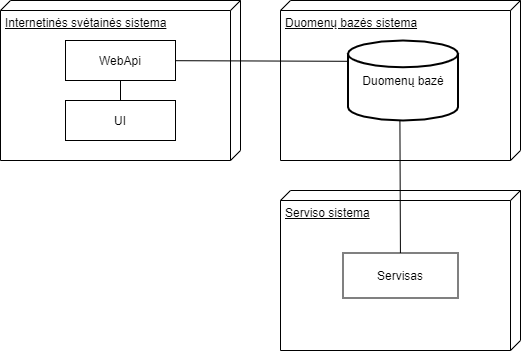
\includegraphics[width=0.9\textwidth]{figs/arch1lt.png}
	\caption{Sistemos architektūros schema}
	\label{fig:arch1}
\end{figure}

Sistemos architektūros schemoje \ref{fig:arch1} pavyzdyje, matome tris sistemas - internetinės svetainės sistemą, duomenų bazės sistemą ir serviso sistemą. Internetinės svėtainės sistemoje veikia pati internetinė svetainė, kurioje vyksta prisijungimas prie sistemos, skenavimo užklausu kurimas, ir skenavimo atąskaitų parsisiuntimas. Duomenų bazės sistemoje veikia pati duomenų bazė, kurios paskirtis yra laikyti skenavimo užklausas ir jų rezultatus, taip pat laikyti prisijungo duomenis. Serviso sistema veikia pats servisas kuris atlieką visa skenavimo logiką ir visą bendravima su skenuojama internetine svetaine. Taip pat bendrauja ir su duomenų baze, iš jos pasiema visus duomenis reikalingus skenavimui ir į ją deda visus skenavimo rezultatus. 

UI aplikacija internės svetainės sistemoje sukurta naudojant Angular. WebApi kuris atsakingas už visą bendravima su duomenų baze bei skenavimo ataskaitų formavima, sukurtas naujant ASP.NET Core. 
Duomenų bazė sukurta naudojant Microsoft SQL. Serviso sistemoje esanti serviso aplikacija sukurta naudojant .NET Core su kuriuo parašyta visa pararelinė skenavimų paleidimo logika ir bendravimas su duomenų baze, Bash scriptus, kurie skirti kurti konteinerius ir vykdyti skenavimus, Docker kuris skirtas kurti konteinerius ir užtikrinti visos sistemos saugumą ir stabilumą. Visos sistemos naudoja Ubuntu 16.04 operacinę sistemą. 

\subsection{Vartotojo sąsaja}

\begin{figure}[H]
	\centering
	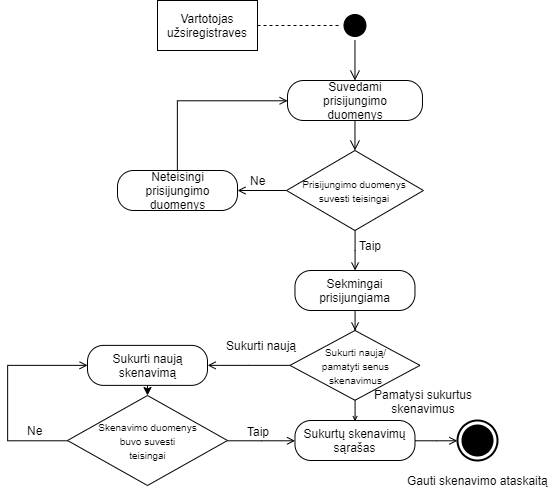
\includegraphics[width=0.9\textwidth]{figs/Activitylt.png}
	\caption{Aktyvumo diagrama}
	\label{fig:activity}
\end{figure}

Aktyvumo diagramoje kuri yra \ref{fig:activity} pavyzdyje, galima matyti visus pasirinkimus kuris vartotojas turi. Vartotojo sąsaja sukurta naudojant Angular, visi atliekami veiksmai keliauja į API kuris sukurtas su ASP.NET Core. API vyksta visa internetinės svetainės logika - autentifikacijos valdymas, bei duomenų valdymas. Jungimosi metu į UI suvedami duomenys keliauja į API, kuriama prisijungimo duomenys yra verifikuojami su duomenų baze. Sekmingai prisijungus, vartotojas gali arba kurti naują skenavimo užklausą, arba pamatyti jau sukurtas. Kuriant skenavimo užklausa, duomenys taip pat yra tikrinami, patikrinus ir sekmingai užregistravus skenavimo užklausa, vartotojas gali eiti į skenavimų sąraša, kur bus pateikta jo sukurtiems skenavimas ataskaitų parsisiuntimo nuorodos, arba jis gali kurti vėl naują užklausą.

\subsection{Saugios aplinkos užtikrinimas}

Internetinių svėtainių skenavimo įrankyje saugi aplinka užtikrinama naudojant Docker, kuris pasižymi tuo, kad su ja yra kuriami konteineriai, kurie yra izoliuoti nuo likusios sistemos. Pačia Docker technologiją galima lyginti su virtualiomis mašinomis kurias pavyzdžiui kuria VirtualBox įrankis. Skirtumas tarp jų vis dėl to yra didžiulis. Docker konteineriai yra kuriami operacinės sistemos lygyje skirtingai negu VirtualBox virtualios mašinos, taip pat kiekviena virtuali mašina turi turėti savo atskirą operacinę sistemą, o konteineriai tiesiog naudoja tapačia opericinę sitema kurioje jie yra kuriami, todėl konteineriai reikalauja žymiai mažiau išteklių, veikia žymiai greičiau, juos galima greitai kurti ir naikinti\cite{merkel2014docker}. Visa tai yra svarbu sistemai, nes kiekvienam procesui yra kuriamas atskirame konteineris, po kiekvieno proceso įgyvendinimo, konteineris yra sunaikinamas. Konteineriu greitis leidžia tai padaryti greitai ir saugiai, nėra priežasties kodėl konteinerius reiktų pernaudoti, nereikia surašinėti atskirai operacinių sistemų ir jas konfiguruoti, taip pat mažas resursu kiekis nestabdo visos sistemos bendrai, ir užtikrina, kad sistemą nesustos veikti.

\subsection{Skenavimo užklausų įgyvendinimas NEPABAIGTA}

\begin{figure}[H]
	\centering
	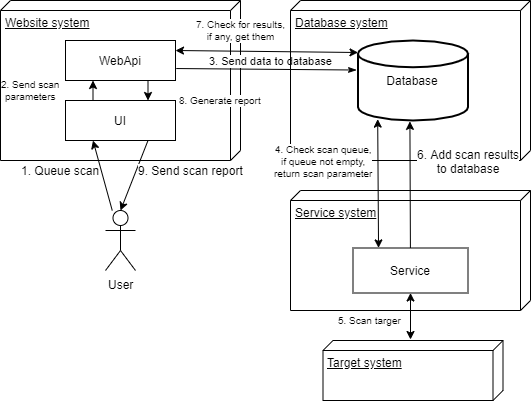
\includegraphics[width=0.9\textwidth]{figs/Full.png}
	\caption{Įrankio pilna veikimo schema}
	\label{fig:full}
\end{figure}

\begin{figure}[H]
	\centering
	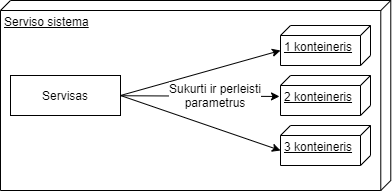
\includegraphics[width=0.9\textwidth]{figs/1Containerlt.png}
	\caption{Konteinerių sukurimas}
	\label{fig:1Container}
\end{figure}

\begin{figure}[H]
	\centering
	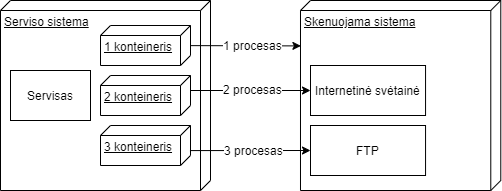
\includegraphics[width=0.9\textwidth]{figs/2Containerlt.png}
	\caption{Proceso Veikimas}
	\label{fig:2Container}
\end{figure}

\begin{figure}[H]
	\centering
	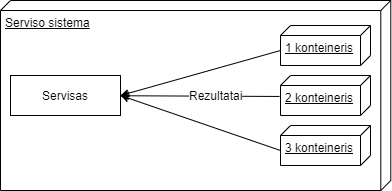
\includegraphics[width=0.9\textwidth]{figs/3Containerlt.png}
	\caption{Rezultatų gražinimas}
	\label{fig:3Container}
\end{figure}

\subsubsection{Igyvendinami skenavimo metodai}



\paragraph{Išorinis sistemos skenavimas}
Išorinis sistemos skenavimas skirtas tam, kad aptiktų atvirus prievadus, patikrinti, kokią informacija išduota pati sistema - kokią operacinę sistemą pati sistema naudoja, kokia tos operacinės sistemos versija, kokios aplikacijos ar sistemos veikia toje sistemoje, ar prie šių sistemų galima jungtis, ar gali prisijungti anoniminei vartotojai. Skenavimo įgyvendinimo metu yra sukuriamas konteineris, iš kurio yra atliekamas skenavimas. Skenavimui pasibaigus yra surenkami rezultatai ir atiduodami servisui, konteineris yra saugiai sunaikinamas, o rezultatai patalpinami į duomenų bazę.
\paragraph{Failų skenavimas}
Internetinės sistemos failų skevimas skirtas tam, kad patikrinti ar į sistemą jau nebuvo isilaužta, ir joje nėra paliktu \textit{malware}. Šis skenavimas yra įgyvendinimas skenavimo užklausos metu. Sukuriamas Docker konteineris, iš kurio naudojant \textit{FTP} prisijungiama prie sistemos. Iš \textit{FTP} direktorijos yra parsiunčiami visi failai į konteineri, tuomet yra generuojami visų failų MD5 maišos žodžiai, kurie yra paruošiami tikrinimui ir yra patikrinami žinomų \textit{malware} failų MD5 maišos žodžių duomenų bazėje. Tuomet rezultatai yra gražinami į servisą, o pats konteineris yra saugiai sunaikinamas. Rezultatai patalpinami į duomenų bazę.
\paragraph{Internetinės svėtainės prieigos skenavimas}
Internetinės svėtainės prieigos skenavimas yra skirtas tam kad aptiktų potencialias \textit{MITM} atakas, \textit{Phishing} svėtaines, \textit{malware} svėtaines. Veikimas yra toks, kad svetainės adresas yra nusiunčiamas trečiajai šaliai, kuri svetainės adresą skenuoja su įvairiomis antivirusinėmis. Tuomet yra pateikiama detali ataskaita. Kadangi šio skenavimo metu nera kontaktuojama su pačia svetaine tiesiogiai, Docker konteineriai nėra kuriami.
\paragraph{Internetinės svėtainės enumeravimas}
Internetinės svėtainės enumeravimas yra skirtas tam, kad aptiktu potencialias internetinės svėtainės spragas tokias kaip atviras direktorijas, kuriose puolėjas gali be jokių kliučių perskaityti jose ęsančių failų turinį. Taip pat aptinkama visi internetinės svetainės puslapiai, prie kurių vartotojas gali prieiti be jokios autentifikacijos, sakykime prie administratoriaus puslapio, šios problemos kyla dėl blogai sukonfiguruotų teisių ar pačio puslapio autentifikacijos. Skenavimo metu yra sukuriamas konteineris, kuriame vykdomas enumeravimas, konteineryje susigeneruoja rezultatų failas, kuris yra gražinamas servisui, o pats konteineris yra saugiai sunaikinamas. Rezultatai yra patalpinami į duomenų bazę.

\subsection{Įrankio Skenavimo metodų platforma}

Įrankis yra puikiai pritaikytas naudoti bet kokioje sistemoje, taip pat jį ypač patogu pritaikyti bet kokia scenarijuje. Šis įrankis yra plačiai naudojamas kibernetinio saugumo bendruomeneje ir taip pat yra ypač efektyvus atliekant tinklo skanavimus ar analizę. Atsisžvelgus į šiuos faktus, šis įrankis tampa butinybė bet kokioje spragų skanavimo sistemoje dėl savo didelio potencialo ir bendruomenės pasitikėjimo.
\begin{algorithm}
	\caption{Įrankio platformos pseudo kodas}
	\label{alg:pseudo}
	\begin{algorithmic}
		\STATE $ScanRequests \gets Database$
		\IF{$ScanRequests > 0$}
		\FORALL {$ScanRequests$}
		\STATE $ThreadPool \gets Scan1(ScanRequest)$
		\STATE $ThreadPool \gets Scan2(ScanRequest)$
		\STATE $ThreadPool \gets Scan3(ScanRequest)$
		\STATE $ThreadPool \gets Scan4(ScanRequest)$
		\STATE $ThreadPool. Wait For All$
		\ENDFOR
		\STATE $Database \gets ThreadPool.Results$
		\ENDIF
	\end{algorithmic}
\end{algorithm}


Įrankio kurimo metu buvo sukurta platforma, kuri yra integruota į patį įranki. Platforma yra skirta lengvai pridėti naujus skenavimo būdus ir funkcijas. Iš šios platformos yra startuojami visi jau esantis skenavimo metodai. Naujų skenavimo metodu pridėjimas vyksta programiškai, bet pati platforma parašyta taip, kad norint pridėti kažka naujo, nereikia programuoti visko per naujo. Šios platformos kodą galime matyti \ref{alg:pseudo} algoritme. Iš pradžių pasiemame visas skenavimo užklausas kurios dar nebuvo vykdytos iš duomenų bazės, tuomet iteruojame per kiekviena iš jų ir parareliai paleisdžiame visus skenavimo metodus. Kai visi skenavimo metodai yra pasileide, laukiame, kol visi jie pasibaigs. Visiems skenavimams pasibaigus, resultatus patalpiname į duomenų bazę.


\subsection{Aptiktini pažeidžiamumai}

Šiuo metu skenavimo įrankis gali aptikti šiuo pažeidžiamumus:
\begin{itemize}
	\item Aptiktinos yra \textit{MITM} atakos tikrinant internetinės svetainės atsakus;
	\item Aptiktinos direktorijos, kurios sąrašo pavidalu gražina savo turinį, taip atsitinka dėl neteisingai sudėtų teisių sistemoje, dėl šio pažeidžiamumo puolėjas atrades šia direktoriją gali be jokių kliučių peržiurėti joje esančius failus;
	\item Aptiktini puslapiai, prie kurių neprisijunges vartotojas neturėtu galimybės prieiti. Kaip pavyzdį galima būtų pateikti prisijungimo vietas prie administratoriaus sąsajos;
	\item Aptiktinkami \textit{Malware} ir infekuoti failai;
	\item Aptinkamos sistemos, kurios veikia skenuojamoje sistemoje;
	\item Aptinkami atidaryti prievadai.
\end{itemize}

\subsection{Įgyvendinti tikslai}
\label{sec:example}
Įgyvendinti šie apsibrėžti tikslai: 
\begin{itemize}
	\item Sukurta svėtainė, kuri leidžia vartotojuj kurti skenavimo užklausas, ir po jų sukurimo, leidžia atsisiusti suformatuotus rezultatus;
	\item Sukurta platforma ir paruoštukai, kurie leidžia lengvai pridėti naujus skenavimo metodus į įrankį;
	\item Sukurta saugi aplinka, kuri leidžia vartotojuj saugiai skenuoti sistemas ir jų failus, nesibaiminant infekuoti pačio įrankio sistemos;
	\item Aptinkami pažeidžiamumų ir pati sistema paruošta naudojimui;
	\item Sugeneruojama ir pateikiama ataskaika kurią lengva suprasti vartotojuj.
\end{itemize}


\subsection{Trūkumai}
\label{sec:example}

Įrankio kurimo metu buvo susidurta su daug problemų ir sunkumų, kurių pasekoje kaikurie planuoti tikslai nebuvo įgendinti. Pats įrankio kurimo procesas yra ypac sudetingas dėl didelio skaičiaus skirtingų technologijų, su kuriomis yra kuriamos internetinės svėtainės, taip pat kiekviena internetinė svetainė skiriasi nuo kitų savo sistemos komponentais, architektūra, naudojamomis technologijomis.

Kurimo metu buvo planuota panaudoti trečios šalies įranki SqlMap. Šio įrankio paskirtis yra ieškoti ar internetinė svetainė yra pažeidžiama \textit{SQL injection} atakoms. Tokio tipo skenavimui reikėtų sukurti internetinės svėtaines puslapių kodo funkciją, kuri svetainės puslapyje iėško dinaminių nuorodų. Šios nuorodos priema parametrus savo nuorodose. Tuomet SqlMap įrankis bando į šiuos parametrus įdeti manipuliuotą tekstą kuris įvykdytų užklausą duomenų bazeje. Šio įrankio funkcionalumo įgyvendinimas šioje skenavimo sistemoje tapo perdaug problematiškas ir laiko užimantis dėl pačios funkcijos kuri ieškotų tokių įveščių internetinėje svėtainėje. Dėl šios priežasties SqlMap funkcionalumo tekta atsisakyti.

Kurimo metu taip pat buvo užsibrežta įgyvendinti statinė analizę. Šis tikslas buvo įgyvendintas nepilnai, patys failai yra tikrinami žinomų \textit{Malware} duomenų bazėje, bet internetinės svėtainės kodas nėra tikrinamas. Šio tikslo tekta atsisakyti ir perkelti statinės analizės technikų įgyvendinimus į ateities darbus. Šio atsisakymo priežastis yra ta, kad kiekvienai programavimo kalbai reikalingas atskiras statinės analizės įgyvendinimas, kieviena kalba yra kitokia ir jos funkcionalumas ir sintaksė yra kitokia, dėl šios priežasties tokio funkcionalumo kurimo kaštai stipriai didėja.


 %Conclusions section
\sectionWithoutNumber{\keyWordConclusions}{conclu}
Išvados bei rekomendacijos.


%ateities darbų gairės, planas/next steps of the work
\sectionWithoutNumber{Ateities tyrimų planas}{future}{Pristatomi ateities darbai ir/ar jų planas, gairės tolimesniems darbams....}

\subsection{Statinė kodo analizė NESKAITYTI}

\subsubsection{Panaudojimas darbe}
\label{sec:data}
Vartotojui davus \textit{FTP} serverio adresą iš jo bus bandoma atsisiūsti išeities kodą. Atsisiuntus sistemos išeities kodą bus atliekama statinė analizė ir taip bus bandoma aptikti spragas ar scenarijus, kurie kelią potencialią grėsmę pačiai sistemai. Tokios grėsmės būtų - įsilaužimas, arba sistemos veikimo paveikimas, sugadinimas. 

\subsubsection{Dinaminė kodo analizė}

\subsubsection{Panaudojimas darbe}
\label{sec:data}
Dinaminė analizė bus taikoma spragų skenavimo sistemoje su kliento sutikimu. Analizės metu, bus bandoma į visas sistemos įvestis pateikti nenumatytu reikšmių, taip išbandant kuo daugiau nenumatytų scenarijų.


\subsubsection{Vidinių pažeidžiamumų skenavimas}

\subsubsection{Panaudojimas darbe}
\label{sec:data}
Įrankio vartotojas savo noru gali pateikti prisijungimus prie sistemos naudojant \textit{SSH} protokolą. Pasinaudojus šia informaciją įrankis prisijungs prie sistemos, ir naudodamas vidinės analizės komponentą, bandys surinkti kuo daugiau informacijos. Surinkus visą galimą informaciją, bus ieškomos potencialios spragos.

 %file References.bib
\referenceSources{References}
%\bibliographystyle{ieeetr}

%% this part is optional
%%\newpage
%%\begin{appendices}


%%\end{appendices}


\end{document}
